In this chapter we will do further analyses of the model results with particular
emphasis on the AttentionSegRank architecture due to its better performance
and explainability. On Section \label{sec:overfit} we will discuss the effects of using semantic segmentation
on neural network  training. Sections \ref{sec:significance} and \ref{sec:relationship} will show a quantitative analysis between
segmentation, attention, and the perception quantification. Section four shows the effect of combining
image features with segmentation. And finally, on section five we will
analyze the implications of this method on model explainability.

\section{Effect of semantic segmentation on learning}
\label{sec:overfit}
As was already mentioned on section \ref{sec:training}, adding a fixed segmentator to
the neural network architecture resulted in a reduction of performance along with a considerable
reduction of overfitting. The behavior was expected when fully replacing the CNN features,
due to the reduced expressiveness of the segmentation and the lack of finetuning, but
unexpectedly, although it is reduced, this behavior persists when combining the fixed
segmentation with the finetuned ResNet50 through the attention layer. We conclude from this
that restricting the attention weights to the shapes and classes given by the segmentation
has a regularizing effect on learning, reducing the model capacity even when the amount of trainable
weights is maintained.

In the case of the PlacePulse dataset this is not a problem since
all traditional deep models suffer of significant overfitting. It remains an interesting research
question  if these behaviors will transfer to other tasks and datasets.

\begin{figure}[ht]
	\begin{center}
	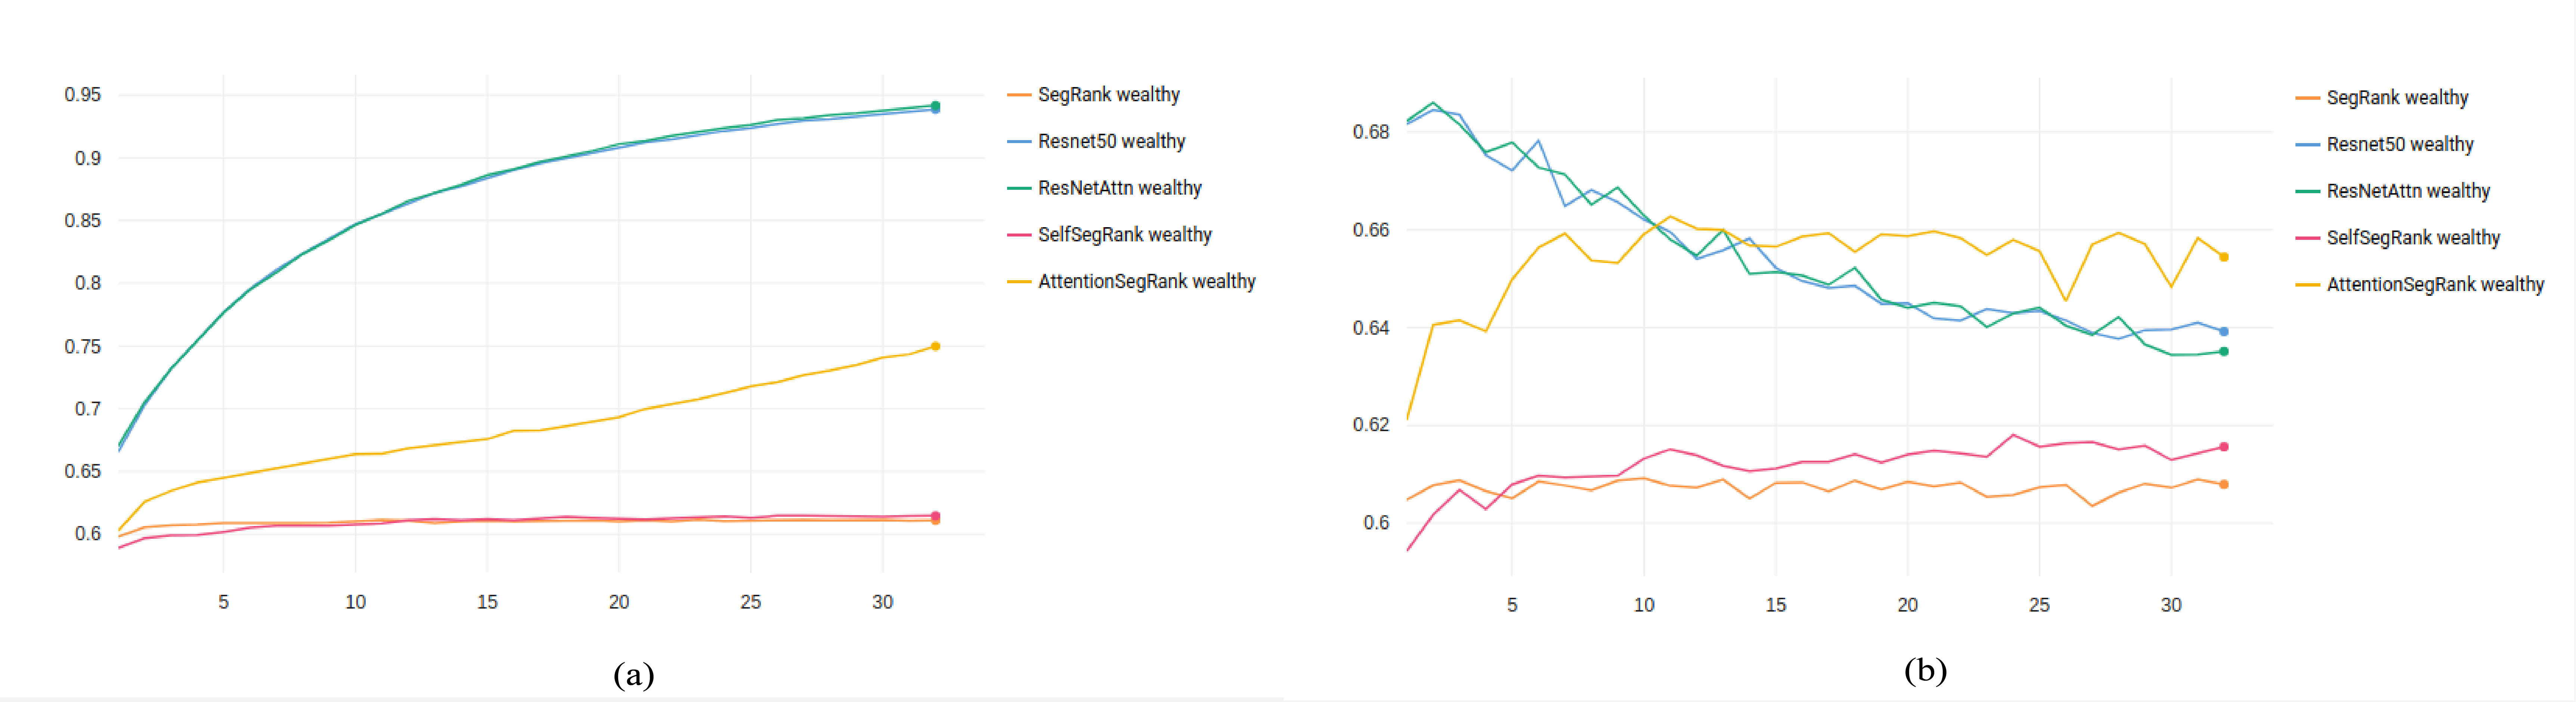
\includegraphics[width=1\textwidth]{./figures/wealthy_graph.png}
	\caption[Wealthy Training curves]{
        Wealthy accuracy vs epoch learning curves on training (a) and validation (b).
        }
	\label{fig:wealthy_graph}
	\end{center}
\end{figure}

\section{Segmentation as an attention subject.}
\label{sec:significance}

By combining the outputs of the segmentation and the attention, we can infer if a certain class was
important for the quantification of perception of a single image. We do this by computing the ratio between
the percentage of pixels belonging to a single class and the percentage of attention placed by the model on
those pixels:
\begin{equation}
	\text{significance ratio} = \frac{\% \text{ attention}}{ \% \text{ segmentation}}
\end{equation}

Using that, we define that a class is significant in an image when significance ratio $\geq 1$,
meaning that the total attention received by the pixels belonging to that class is larger
than the amount they would get if the attention was distributed uniformly over the whole image.

We calculate the significance of all the CityScapes classes
on all the images of the validation split for each of the perception attributes. We show
the results for the most significant classes on figures \ref{fig:total_sig} and \ref{fig:presence_sig}, which show the percentage
of images where each class is considered significant, over the whole split or filtered by the images
where the class is present respectively. For the full results see appendix \ref{sec:sig_tables} .

\begin{figure}[ht]
	\begin{center}
	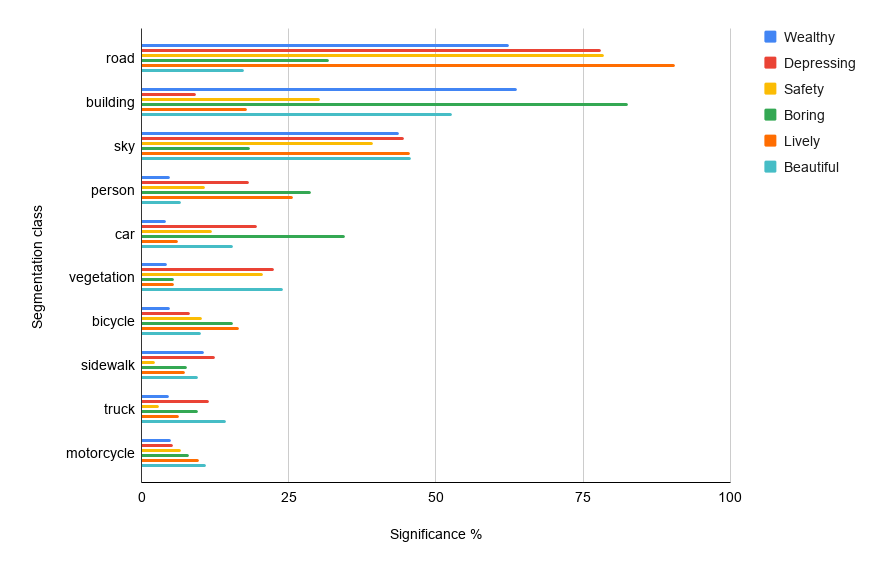
\includegraphics[width=1\textwidth]{./figures/total_significance.png}
	\caption[Percentage of class significance when total]{
		Percentage of times a segmentation class is considered significant over the whole dataset, for the
		10 most significant classes on average.
        }
	\label{fig:total_sig}
	\end{center}
\end{figure}

\begin{figure}[ht]
	\begin{center}
	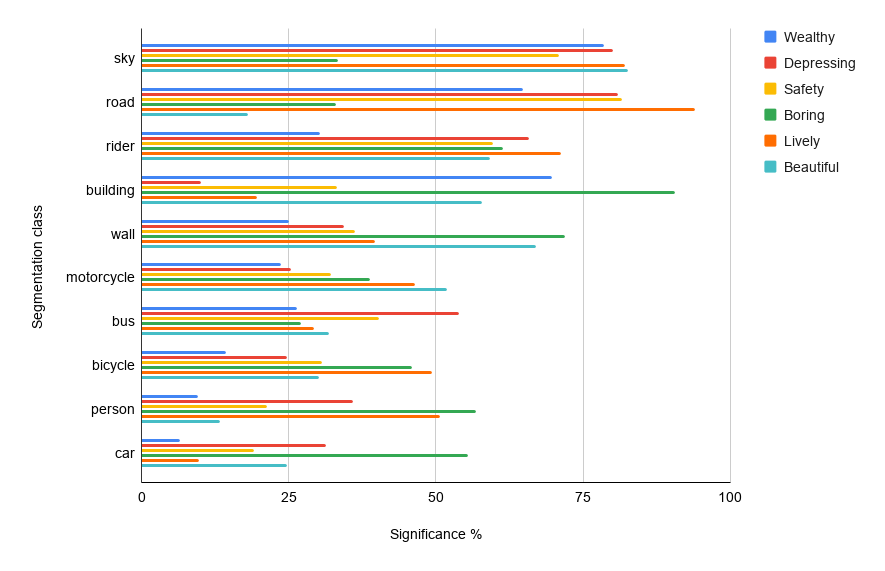
\includegraphics[width=1\textwidth]{./figures/present_significance.png}
	\caption[Percentage of class significance when present]{
		Percentage of times a segmentation class is considered significant when it is present in an image, for the
		10 most significant classes on average.
        }
	\label{fig:presence_sig}
	\end{center}
\end{figure}


The most notable insight from this results is that there are considerable differences on the same class
but for different attributes, for example buildings are the most significant for the boring attribute
but is one of the least for the depressing attribute. Vegetation is significant for beautiful and
depressive but not for wealthy. Another insight is that some classes are on average considerably more significant
than others, we believe this happens because they are much more common than others in the dataset
and the networks learn to consider them more often. For the exact distribution of the segmentation classes
see appendix \ref{sec:seg_distribution}.

Even though the  set of classes used by \citeA{zhang_measuring} is not exactly the same as
the one we use in our study, the most significant classes for our model are consistent with
the ones presented in their regression model. This is important because it shows we
are approaching the interpretability of regression model with a considerably larger
neural network.

These results support that attention weights are a good way to augment the explainability of
the models since they show that the same architecture learns to attend to different things
when quantifying different attributes.


We can also visualize which classes are significant for individual examples, allowing
for a simple interpretation of results on a per instance basis.
See figure \ref{fig:ratio} in which the road and sky classes were determined as significant
by the models attention.

\begin{figure}[ht]
	\begin{center}
	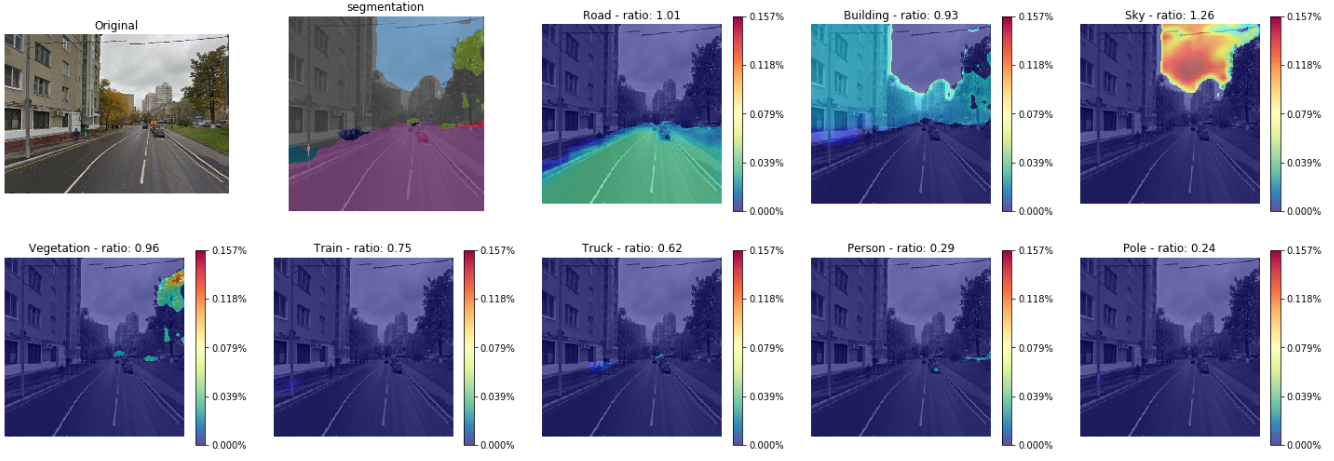
\includegraphics[width=1\textwidth]{./figures/ratio.png}
	\caption[Example of significance ratio]{
        Sample visualization including class significance for the safety attribute.
        }
	\label{fig:ratio}
	\end{center}
\end{figure}


\section{Relationship between urban perception and semantic segmentation}
\label{sec:relationship}

Similarly to previous work \cite{rossetti, zhang_measuring} we analyze how the segmentation correlates with the quantified
perception scores. For that, we count the percentage of pixels of each segmentation class
on all the images of the validation split for each of the perception attributes and measure
correlation with the perception quantification. We present these results for both
segmentation and attention percentages on figure \ref{fig:correlations}.

In all classes correlation is not extremely high, we believe that to be a good result since
no class should have such a determinant inherence on the perception of an attribute as to
reach a correlation close to 1 or -1. Attention and segmentation behave similarly, having
opposite sign only on very rare cases, (e.g: road for the lively attribute) and differing
only on the magnitude of the correlation most of the time. Comparing with the significance results shown
on figure \ref{fig:total_sig}, the most significant classes on the dataset are also consistently on
the top or bottom of the correlation charts, so the high significance comes hand in hand with
high correlation more often than not.

As is expected, the model's outputs correlate with the classes differently depending on the attribute,
making sense with how the attributes themselves are correlated, for example vegetation is very positive
for beauty but very negative for depressiveness.

\begin{figure}[ht]
	\centering
	\subfloat[wealthy]{
	  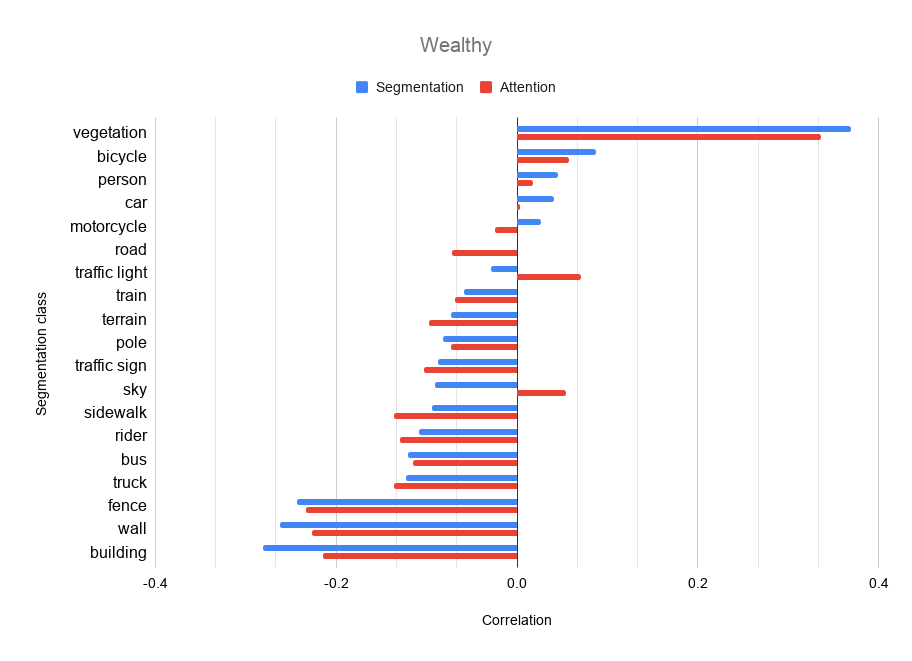
\includegraphics[width=0.45\textwidth]{./figures/wealthy_correlation.png}
	  \label{fig:correlations:wealthy}
	}
	\subfloat[depressing]{
	  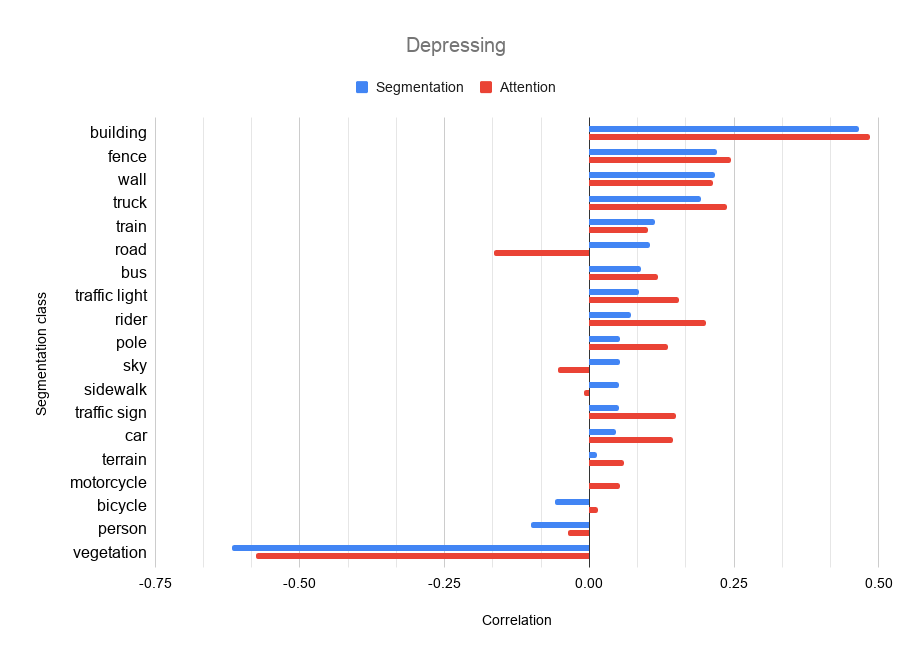
\includegraphics[width=0.45\textwidth]{./figures/depressing_correlation.png}
	}
	\hspace{0mm}
	\subfloat[safety]{
	  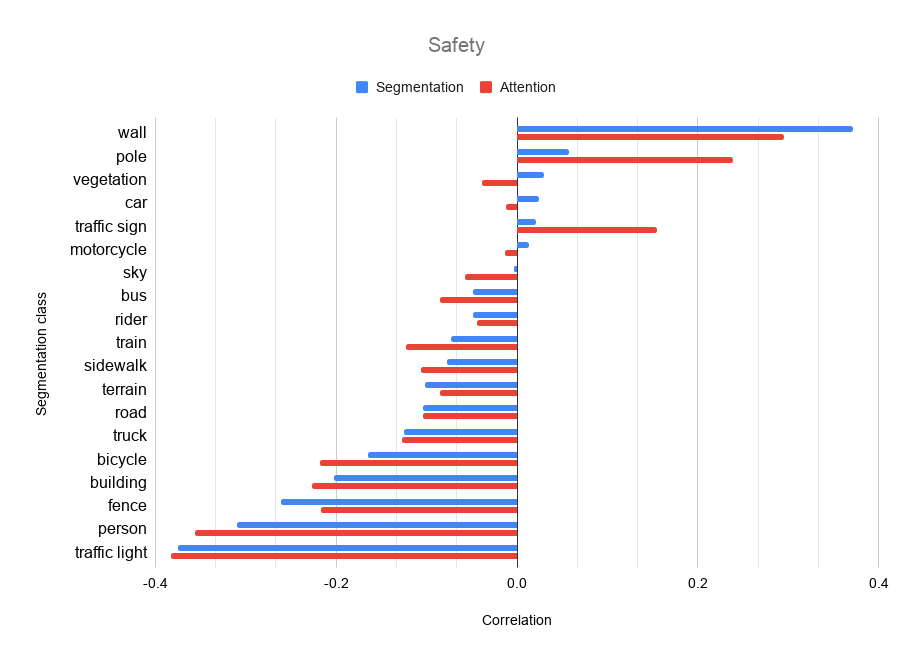
\includegraphics[width=0.45\textwidth]{./figures/safety_correlation.png}
	}
	\subfloat[boring]{
	  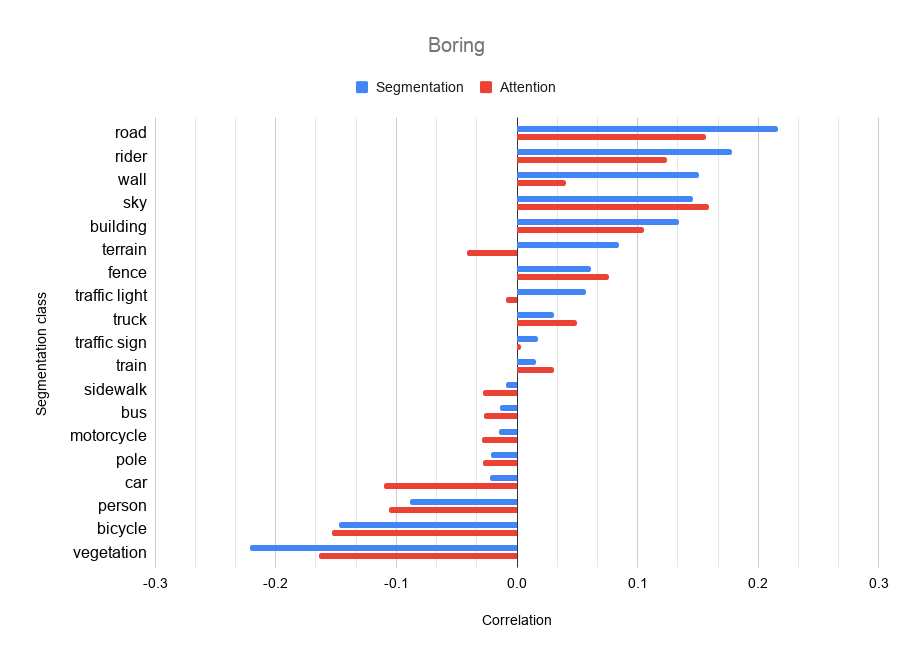
\includegraphics[width=0.45\textwidth]{./figures/boring_correlation.png}
	}
	\hspace{0mm}
	\subfloat[lively]{
	  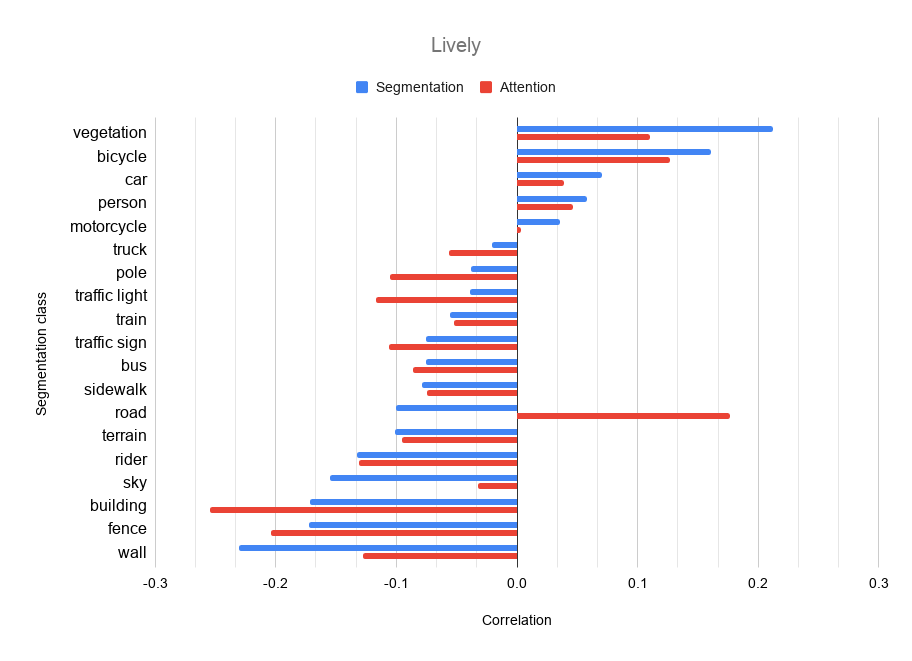
\includegraphics[width=0.45\textwidth]{./figures/lively_correlation.png}
	}
	\subfloat[beautiful]{
	  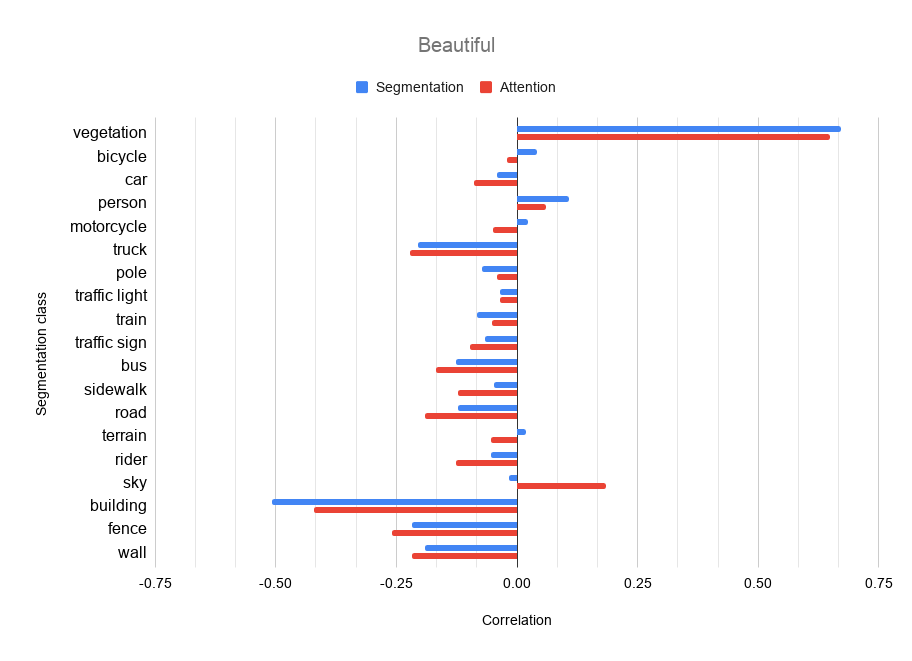
\includegraphics[width=0.45\textwidth]{./figures/beautiful_correlation.png}
	}
	\caption{
		Correlation between segmentation and attention percentages for each class and
		quantified scores.
		}
\end{figure}
\label{fig:correlations}

We also compute correlation between segmentation and score when the respective class is
considered significant by the attention weights. The results are mostly maintained but with
a slight tendency to have larger correlation magnitude. Figure \ref{fig:correlation_significant}
shows an example comparing the correlation for all the images and filtered for significance.
Most classes get an increase in magnitude while keeping the sign fixed. Sign changes can happen
occasionally for classes with very low correlation magnitude ($< 0.1$).

\begin{figure}[ht]
	\begin{center}
	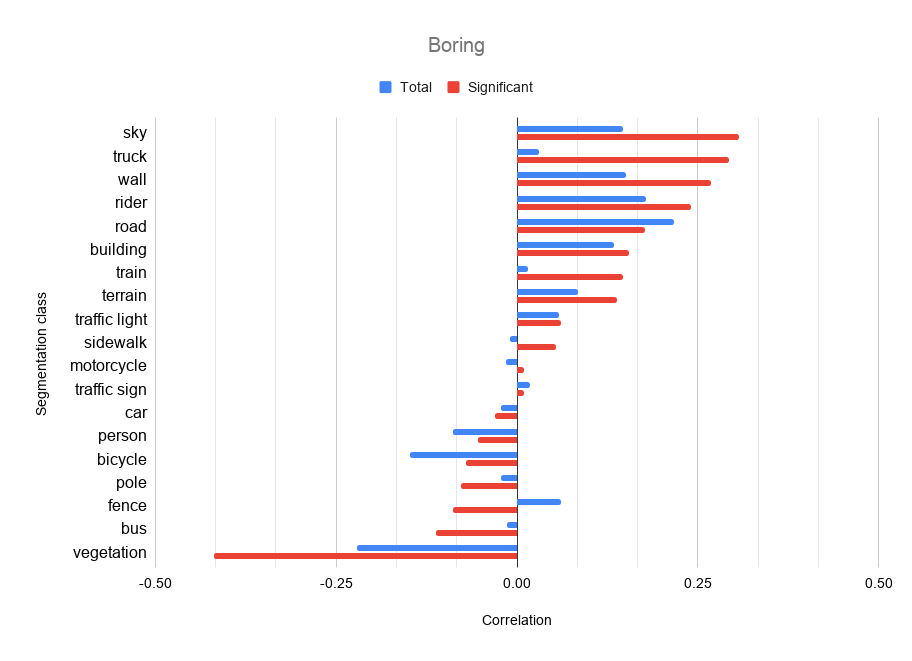
\includegraphics[width=0.75\textwidth]{./figures/boring_correlation_significant.png}
	\caption[Correlation comparison for significant images]{
		Correlation between score and segmentation percentage. Comparison between
		the whole dataset and filtering each class
		by significance. Example for the boring attribute.
        }
	\label{fig:correlation_significant}
	\end{center}
\end{figure}

\begin{figure}[ht]
	\centering
	\subfloat[vegetation]{
	  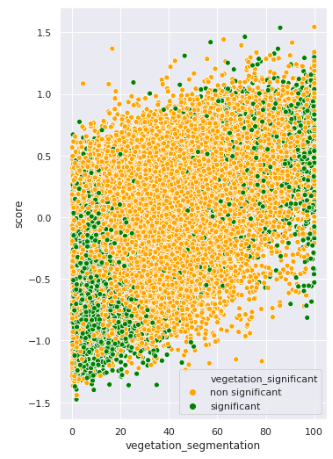
\includegraphics[width=0.3\textwidth]{./figures/vegetation_scatter.png}
	}
	\subfloat[building]{
	  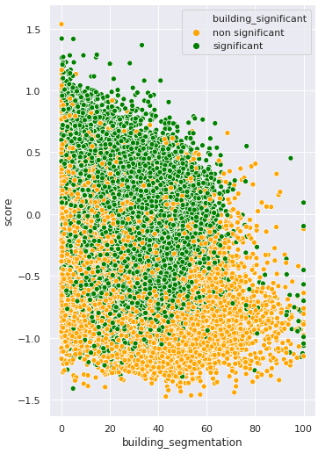
\includegraphics[width=0.3\textwidth]{./figures/building_scatter.png}
	}
	\hspace{0mm}
	\subfloat[fence]{
	  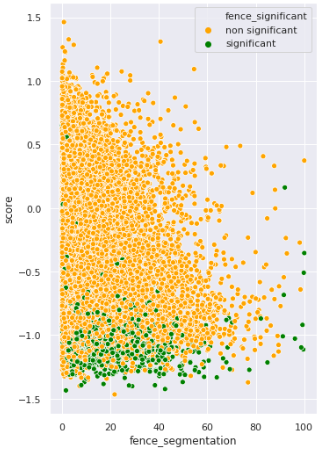
\includegraphics[width=0.3\textwidth]{./figures/fence_scatter.png}
	}
	\caption[Score vs segmentation scatter plots]{
		Scatter plots for the 3 classes with highest correlation for the beautiful attribute.
		Colors denote if that class was significant for that image.
	}
	\label{fig:scatters}
\end{figure}

Even though some classes have high (or low) correlation is important to note that in no case
their sole values are enough to determine the final output score, even when filtering by significance.
Other objects on the images and ResNet features are also necessary to get a more precise
quantification of the perception. See figure \ref{fig:scatters} where even though the correlation
can be seen clearly, for a single segmentation percentage the scores fall over a large interval.

As we mentioned above, \citeA{zhang_measuring} used different segmentation classes
in their study so an exact comparison of results is not possible. However the correlations we obtained
are mostly consistent in sign and in order of magnitude with the beta coefficients they
obtained (see figures \ref{fig:correlations} and \ref{fig:beta}).

Some interesting insights can be drawn from the correlation results:

\begin{itemize}
	\item Buildings have a general "negative" connotation, making images more depressing and
	boring, and less wealthy, safe, lively and beautiful.
	\item Vegetation is the opposite, making images more wealthy, lively and beautiful and less
	depressing and boring.
	\item Unlike \cite{rossetti} we find that fences have a general "negative" connotation,
	similar to buildings.
	\item People make images feel less safe, but also less boring.
	\item Bicycles, which are rarely present in the dataset, are very discriminative for
	many attributes.
	\item Even though it has high attention weights on a large percentage of the images, the sky doesn't have
	a clear tendency on most attributes, excepting for boring.
\end{itemize}

\section{Effect of combining features and segmentation.}
\label{sec:combining}

As a way of ablation study we evaluate the same metrics with the more basic models.
By analyzing SelfSegRank and AttentionSegRank we can see the impact the ResNet features have on the model  behavior
besides the performance improvement.
Using only segmentation results in a larger bias in significance towards the classes more
common in the dataset, with the least present reaching 0\% significance for some attributes.
Following that tendency, the correlation order of the classes is mostly kept, but with an
increase in the correlation magnitude, that is an expected behavior since this model depends on segmentation as
the sole input. An example of this difference can be seen on figure \ref{fig:correlation_comparison}  or
by comparing figure \ref{fig:correlation_selfsegrank} and figure \ref{fig:correlations:wealthy}.

Another interesting behavior of the segmentation only architectures is
that when a single segmentation class takes a large portion of an image,
the model output tends to converge to a middle point value. This may be due to the lack of
information the model has when the inputs consists solely of a large  blob of a single class with no
additional features. The fact that this behavior is not replicated by the AttentionSegRank model, supports
that adding the traditional image features to the segmentation is a better approach not only for performance
but for explainability as well.

\begin{figure}[ht]
	\begin{center}
	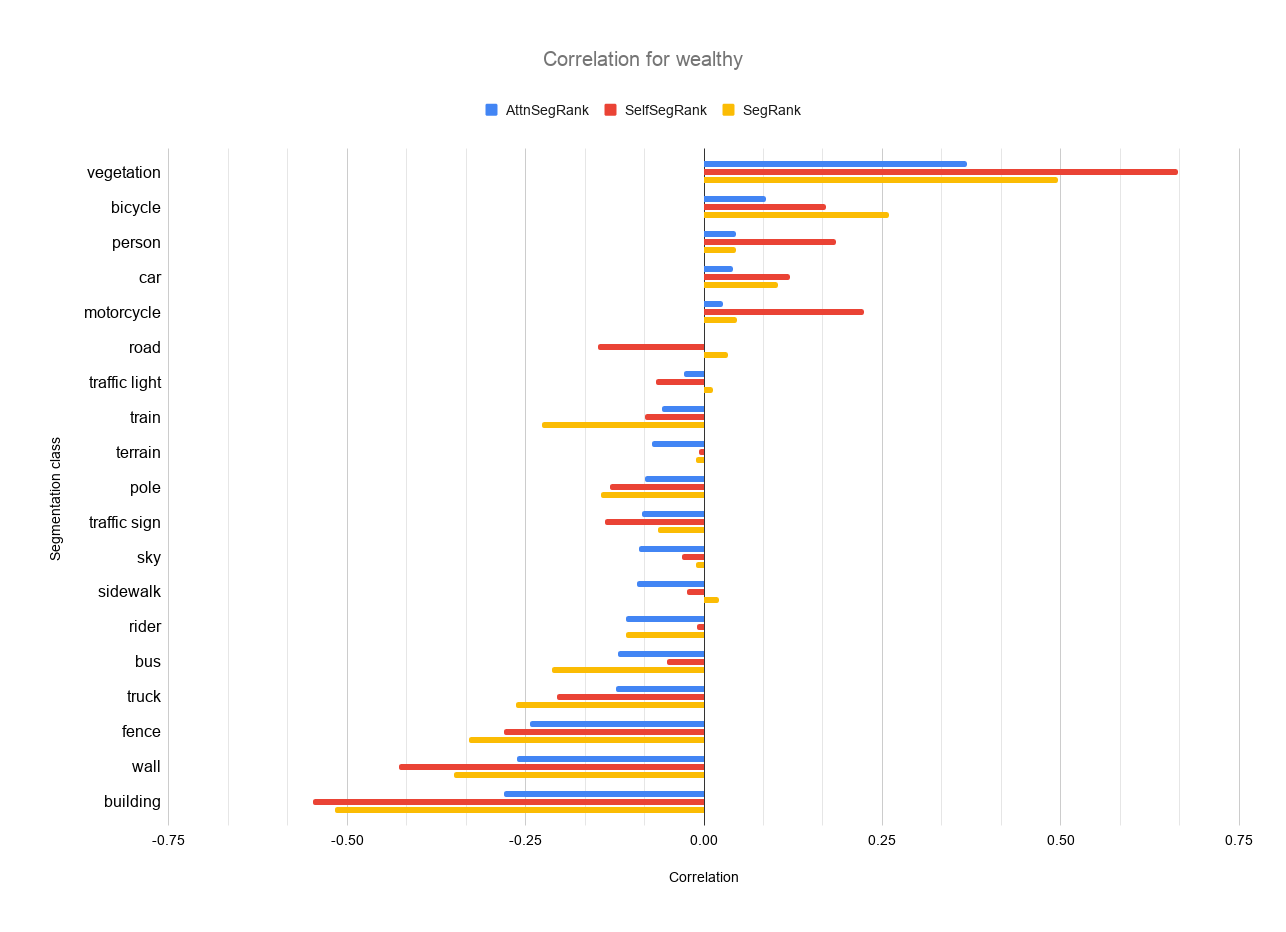
\includegraphics[width=0.75\textwidth]{./figures/correlation_comparison.png}
	\caption[Correlation comparison]{
		Segmentation and score correlation comparison for the three architectures on the wealthy
		attribute.
        }
	\label{fig:correlation_comparison}
	\end{center}
\end{figure}

\begin{figure}[ht]
	\begin{center}
	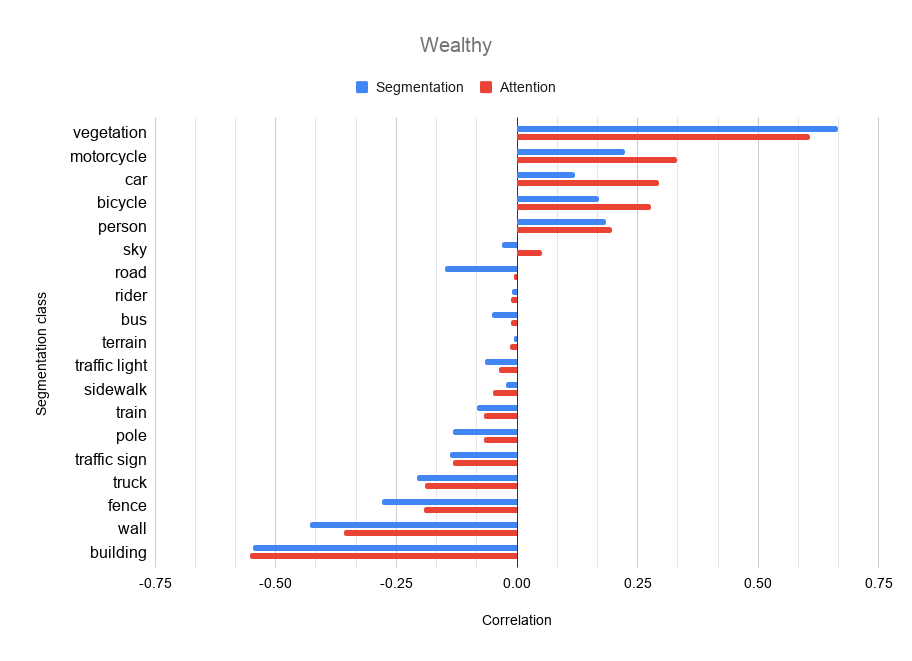
\includegraphics[width=0.75\textwidth]{./figures/selfsegrank_correlation.png}
	\caption[SelfSegRank Correlation]{
		Correlation between score and segmentation/attention percentages on the
		SelfSegRank model. Example for the SelfSegRank architecture on the wealthy attribute.
        }
	\label{fig:correlation_selfsegrank}
	\end{center}
\end{figure}

\begin{figure}[ht]
	\centering
	\subfloat[building]{
	  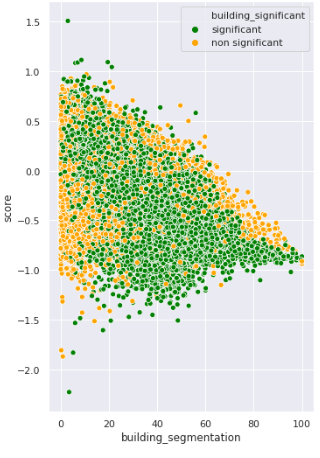
\includegraphics[width=0.3\textwidth]{./figures/building_scatter_selfsegrank.png}
	}
	\subfloat[truck]{
	  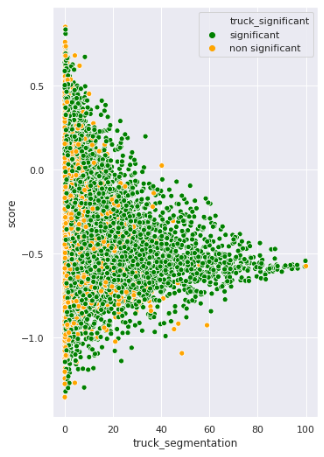
\includegraphics[width=0.3\textwidth]{./figures/truck_scatter_selfsegrank.png}
	}
	\hspace{0mm}
	\subfloat[sky]{
	  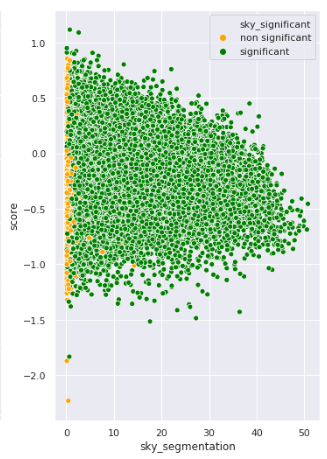
\includegraphics[width=0.3\textwidth]{./figures/sky_scatter_selfsegrank.png}
	}
	\caption[SelfSegRank score vs segmentation scatter plots]{
		Scatter plots showing examples of converging attributes on the SelfSegRank model. All plots made
		for the wealthy attribute.
	}
	\label{fig:scatters_selfsegrank}
\end{figure}

\section{Effect of attention over semantic segmentation on model explainability.} \label{sec:seg_explainability}
The main objective of this work is to improve model explainability. The tool we present
towards that objective is the use of semantic segmentation to compute attention weights. This
approach generates considerably better attention weights from a semantic standpoint, since
the shapes generated have a very high consistency with those given by the semantic segmentation,
which are by definition human understandable.

Models in the computer vision literature that use attention
weights to enhance explainability have the constant
problem of region boundaries not being clearly delimited, often having
shapes that do not resemble any human known object or figure in the image
\cite{zhang_interpretable,zhang_relation,johnston_depth,carion_object}.
Figure \ref{fig:model_comparison} shows an example
of the advantage of our method over the baseline, which consists of
a traditional attention mechanism.

Another benefit of segmentation based attention weights
is, since weights have a human understandable shape,
we can also analyze how they behave visually
in an aggregated way, we do that by calculating the mean
attention of each pixel belonging
to a class through out the whole dataset, and use them to
generate visualizations for each class and attribute.
This visualizations allow  for an spatial analysis for
different attributes, for example on figure \ref{fig:average_vegetations},
there is a clear distinction between some attributes attending the top parts
and others the bottom parts of image, this makes sense considering the vegetation
class includes both trees (upper half) and grass and bushes (bottom half) which
have different incidence depending on the attribute. This result
is consistent with the previous literature \cite{rossetti, zhang_measuring}.

\begin{figure}[ht]
	\centering
	\subfloat[wealthy]{
	  
\includegraphics[width=0.3\textwidth]{./figures/vegetation_averages/wealthy.png}
	}
	\subfloat[depressing]{
	  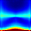
\includegraphics[width=0.3\textwidth]{./figures/vegetation_averages/depressing.png}
	}
	\hspace{0mm}
	\subfloat[safety]{
	  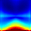
\includegraphics[width=0.3\textwidth]{./figures/vegetation_averages/safety.png}
	}
	\subfloat[boring]{
	  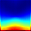
\includegraphics[width=0.3\textwidth]{./figures/vegetation_averages/boring.png}
	}
	\hspace{0mm}
	\subfloat[lively]{
	  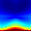
\includegraphics[width=0.3\textwidth]{./figures/vegetation_averages/lively.png}
	}
	\subfloat[beautiful]{
	  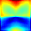
\includegraphics[width=0.3\textwidth]{./figures/vegetation_averages/beautiful.png}
	}
	\caption[Vegetation attention averages]{
		Attention averages for the vegetation class. Red means more attention. The color
		scales are logarithmic and are different for each image to ensure all the visualizations
		are clear.
		}
\label{fig:average_vegetations}
\end{figure}

Another interesting case to analyze is the road class, shown in figure \ref{fig:average_road}.
As expected the average attentions show a triangular shape on the bottom of the images, which
is how the road is shown in most images, but the boring and beautiful attributes put more attention
on the top of the images, which only happens on images that are mostly road, such as tunnels and
highways, combining this with the fact that road correlates negatively with beautiful and very
positively with boring, we can see that the results are reasonable since highways and tunnels are
indeed not so beautiful and quite boring.

\begin{figure}[ht]
	\centering
	\subfloat[wealthy]{
	  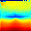
\includegraphics[width=0.3\textwidth]{./figures/road_averages/wealthy.png}
	}
	\subfloat[depressing]{
	  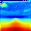
\includegraphics[width=0.3\textwidth]{./figures/road_averages/depressing.png}
	}
	\hspace{0mm}
	\subfloat[safety]{
	  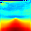
\includegraphics[width=0.3\textwidth]{./figures/road_averages/safety.png}
	}
	\subfloat[boring]{
	  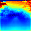
\includegraphics[width=0.3\textwidth]{./figures/road_averages/boring.png}
	}
	\hspace{0mm}
	\subfloat[lively]{
	  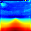
\includegraphics[width=0.3\textwidth]{./figures/road_averages/lively.png}
	}
	\subfloat[beautiful]{
	  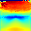
\includegraphics[width=0.3\textwidth]{./figures/road_averages/beautiful.png}
	}
	\caption[Road attention averages]{
		Attention averages for the road class. Red means more attention. The color
		scales are logarithmic and are different for each image to ensure all the visualizations
		are clear.
		}
\label{fig:average_road}
\end{figure}
